
%\chapter{多语言模型系统中基于角色的交互}\label{chap:roleint}\label{chap:role}

\chapter{多语言模型系统中基于角色的交互}\label{chap:roleint}\label{chap:role}

\begin{learningbox}
本章将介绍多个大语言模型智能体在被赋予角色、并在群体中交互时的行为。具体而言，你将能够：
\begin{itemize}[leftmargin=*, nosep]
    \item 区分{\em 基于角色的}多智能体交互（本章）与{\em 开放式}涌现式仿真（第~\ref{chap:emergent} 章）。
    \item 描述大语言模型智能体在{\em 博弈论}设定中彼此交互时的行为，并将其与单智能体的策略性发现（第~\ref{chap:behavior} 章）联系起来。
    \item 解释{\em 基于角色的协作模式}，并识别实现它们的框架。
    % \item Describe how agents are coordinated in practice, distinguishing orchestrator--worker from peer-to-peer topologies, and name the protocols used to connect them.
    \item 批判性地评估多智能体协作何时改善表现、何时不能，以及多智能体交互引入了哪些新的失效模式与{\em 安全风险}。
\end{itemize}
\end{learningbox}

\section{从单智能体到多智能体}
上一章从行为视角研究了个体大语言模型与由大语言模型驱动的智能体：单个模型如何解读交流、社会或道德情境，并在其中行动。本章从单智能体转向多智能体设定，考察当若干基于大语言模型的智能体被迫交互时会发生什么，例如作为博弈论竞赛中的对手、以及作为团队中的协作者。分析单位从单个模型的行为画像，转向模型之间产生的交互模式与集体结果。

\subsection{多智能体仿真：历史与现状}
用人工智能体研究交互在计算社会科学中有着悠久历史 \citep{epstein1996growing,macal_tutorial_2010}。传统上，具备基本感知、推理与决策能力的智能体群体在虚拟环境（在基于机器人的仿真中则是真实环境）中交互 \citep{steels1995self,shoham2008multiagent}。这类仿真的目的通常是把理论工作与实验工作衔接起来，在真实世界实验困难或昂贵的领域中，用人工行为作为人类行为假设的检验场。

历史上曾有两个障碍限制这条研究路线：难以验证行为是否逼真，以及仿真智能体社会的高昂计算成本。智能体式大语言模型与仿真基础设施的进展 \citep{rutherford2024jaxmarl} 正在改变这一局面。基于大语言模型的智能体用自然语言交流，能处理丰富的背景知识，还能被赋予差异化的人格设定，使仿真交互更具表现力，也更可直接与人类交互相比。

\subsection{基于角色的交互与涌现式交互}
多语言模型研究可以按研究者对仿真的控制程度来分类。在一端，每个智能体都被赋予一个\emph{角色}，其形式为人格设定、目标与交互协议。研究问题通常是智能体在被指定的结构中如何行为，以及由此形成的系统整体表现如何——与其他被指定的结构与角色相比。在另一端，智能体被置于没有预先角色分配的开放环境中，研究问题是\emph{涌现}出什么社会结构：群体动力学、惯例与规范。本章关注这一谱系中基于角色的一端，第~\ref{chap:emergent} 章讨论涌现侧。

这一区分对方法论选择与结果解读都很重要。在基于角色的系统中，角色与交互协议是设计决策或实验变量。行为是相对于系统被设计的目标来评估和解读的。在涌现式设定中，目标或任务只在背景中起作用（或完全不存在）。分析更为开放和探索性，更接近民族志而非基准评测。不过，后面会清楚看到，这一区分并非绝对：基于角色的系统常常表现出它们并非被设计出来的行为。

\subsection{多智能体协作的五个维度} \label{fivedimensions}
作为本章的组织原则，我们采用 \citet{tran2025multi} 的分类，沿大语言模型协作的五个维度展开：
\begin{enumerate}
    \item \emph{行动者}：涉及的智能体，以及它们是同质的（同一模型的多个实例）还是异质的（不同模型或能力画像）
    \item \emph{交互类型}：合作、竞争，或两者的混合（「竞合」）
    \item \emph{结构}：智能体如何组织，例如点对点、集中式或分布式
    \item \emph{策略}：如何引出协作，例如通过角色分配或通过模型层面的机制
    \item \emph{协调协议}：把智能体绑定在一起、并规范其通信的机制
\end{enumerate}
本章讨论的系统在这五个轴上做出不同选择，牢记这些维度有助于看清每个框架新在何处。

\subsection{一点方法论提醒}
评测多智能体系统继承了评测单个模型的每一项方法论困难：提示敏感性、测试材料可能泄露进训练数据、采样变异性。此外，它还带来了自身的新困难：
\begin{itemize}
    \item 所报告的结果往往更难复现，因为某个智能体输出中的微小变化会级联影响后续交互，增加运行间变异。
    \item 表现差异的成因可能不清楚：是多智能体协作本身、协调协议、为角色分配而嵌入的提示工程，还是多个智能体累积消耗的额外推理预算。
    \item 构念效度转移到社会—交互术语这一层面：{\em 团队协作}、{\em 讨论}、{\em 集体决策}等概念承载着丰富的人类内涵，而实际仿真未必配得上这些内涵。
\end{itemize}
带着这些告诫，本章先讨论最简单的多智能体设定：大语言模型智能体在策略性场景中彼此对阵，除博弈本身之外不分配任何角色（第~\ref{sec:strat} 节）。接着，我们考察当通过定义协调协议与明确角色来理顺交互时，什么发生了变化（第~\ref{sec:roletask} 节）。


\section{大语言模型智能体之间的策略性交互} \label{sec:strat}
在第~\ref{chap:behavior} 章中，我们考察了大语言模型在被提示与脚本化对手进行经济博弈时的行为。这里我们考虑{\em 大语言模型智能体彼此交互}的博弈论场景研究。本节中的智能体是对称的同侪：各自追求自身利益，没有任何一个被赋予协调或监督角色。我们先看同时跨多个博弈给大语言模型智能体打分的基准，再看围绕单一场景构建的更丰富的仿真平台中的行为。

\subsection{跨博弈的策略能力基准评测}
MAgIC 研究 \citep{xu2024magic} 使用社交推理游戏（谁是卧底、变色龙）以及成本分摊、多人囚徒困境、公共品博弈等博弈论场景。目标是提取七种能力：理性、判断、推理、欺骗、自我意识、合作与协调，如图~\ref{fig:radar} 所示。现成形态与增强形态的大语言模型在多智能体设定中接受这些能力的评估。

GPT-o1 与 GPT-4 的得分显著优于其他模型。大语言模型在判断、理性与合作上普遍得分较高，部分模型在欺骗上也较高，但在推理上较低，且除一个模型外，所有模型在协调上都得分低。唯一的例外是结合概率图建模的 GPT-o1——这是受 \citet{kollerfriendman2009pgm} 启发的一种类心理理论能力的实现。作者表明，概率图建模能全面提升大语言模型的表现。这与第~\ref{sec:theoryofmind} 节讨论的一般证据一致：人类在策略性场景中严重依赖心理理论。

\begin{figure}
  \begin{center}
    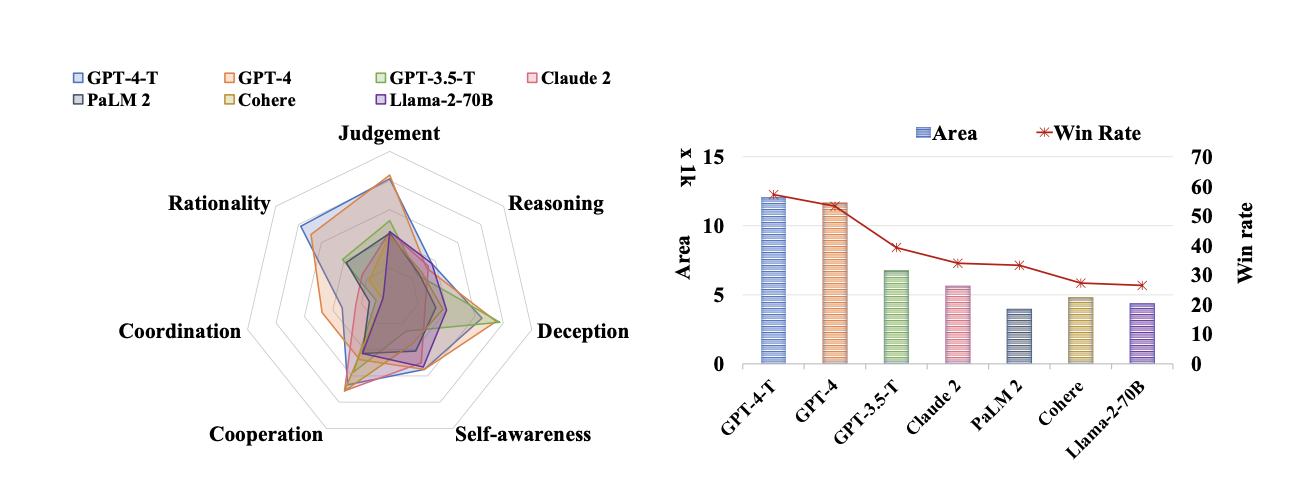
\includegraphics[width=\textwidth]{figures/radar}
    \caption{大语言模型在各项指标上的表现 \citep{xu2024magic}}\label{fig:radar}
  \end{center}
\end{figure}

一个把协调本身作为研究对象、而非若干特质之一的基准是 LLM 协调基准 \citep{agashe2025llm}。大语言模型在两项不同任务上接受评估：纯合作博弈中的智能体式协调，以及关于这些博弈的问答（见图~\ref{fig:agashe}）。实验发现，只要决策能依赖环境变量，大语言模型智能体就表现良好；而当成功需要主动推理搭档的信念与意图时，表现就很差。具体来说，这类环境变量包括游戏布局、物体位置、每个智能体当前所处位置、哪些门是开着的等等。最清晰的例证是 Overcooked-AI，这是大语言模型表现最好的游戏。该游戏完全可观测，其动作空间由{\em 从 1 号洋葱分发器取一个洋葱}、{\em 把洋葱放到 0 号盘子}之类的动作构成。在多数场景与布局下，大语言模型只需依据游戏环境的状态考虑接下来最好的步骤，无需考虑其他智能体的视角。

当把 Overcooked 上的表现与 Hanabi 的得分相比时，这种不对称尤其明显——在 Hanabi 中，每个动作都要求推理搭档的信念。在 Overcooked 上，零样本大语言模型智能体可以追平甚至超过专门训练的强化学习基线模型。而在 Hanabi 上，强化学习基线接近满分，多数大语言模型智能体却几乎拿不到分。最好的大语言模型智能体（基于 GPT-4-turbo）也只能达到最高分的一半左右，即便加上显式的心理理论推理与自我验证步骤也是如此。若没有这些增强，GPT-4-turbo 等强模型的得分几乎完全崩塌，说明所测得的这一能力部分是智能体框架的特征，而不只是模型本身的特征。大语言模型智能体在交叉对局中确实更稳健：强化学习方法面对没见过的搭档时表现急剧下降，而大语言模型智能体的零样本特性使其能迁移到没见过的搭档而不损失表现。

该研究的问答部分（见图~\ref{fig:agashe} 右栏）把问题拆解为分别针对环境理解、心理理论与联合规划。他们发现大语言模型在第一类上普遍得分高（最佳模型 >80\%），在心理理论上较低，在联合规划上最差（最佳模型 <40\%，开源模型低于随机水平）。这与在 Overcooked（环境驱动）与 Hanabi（心理理论与规划驱动）之间观察到的得分差异一致。

\begin{figure}
  \begin{center}
    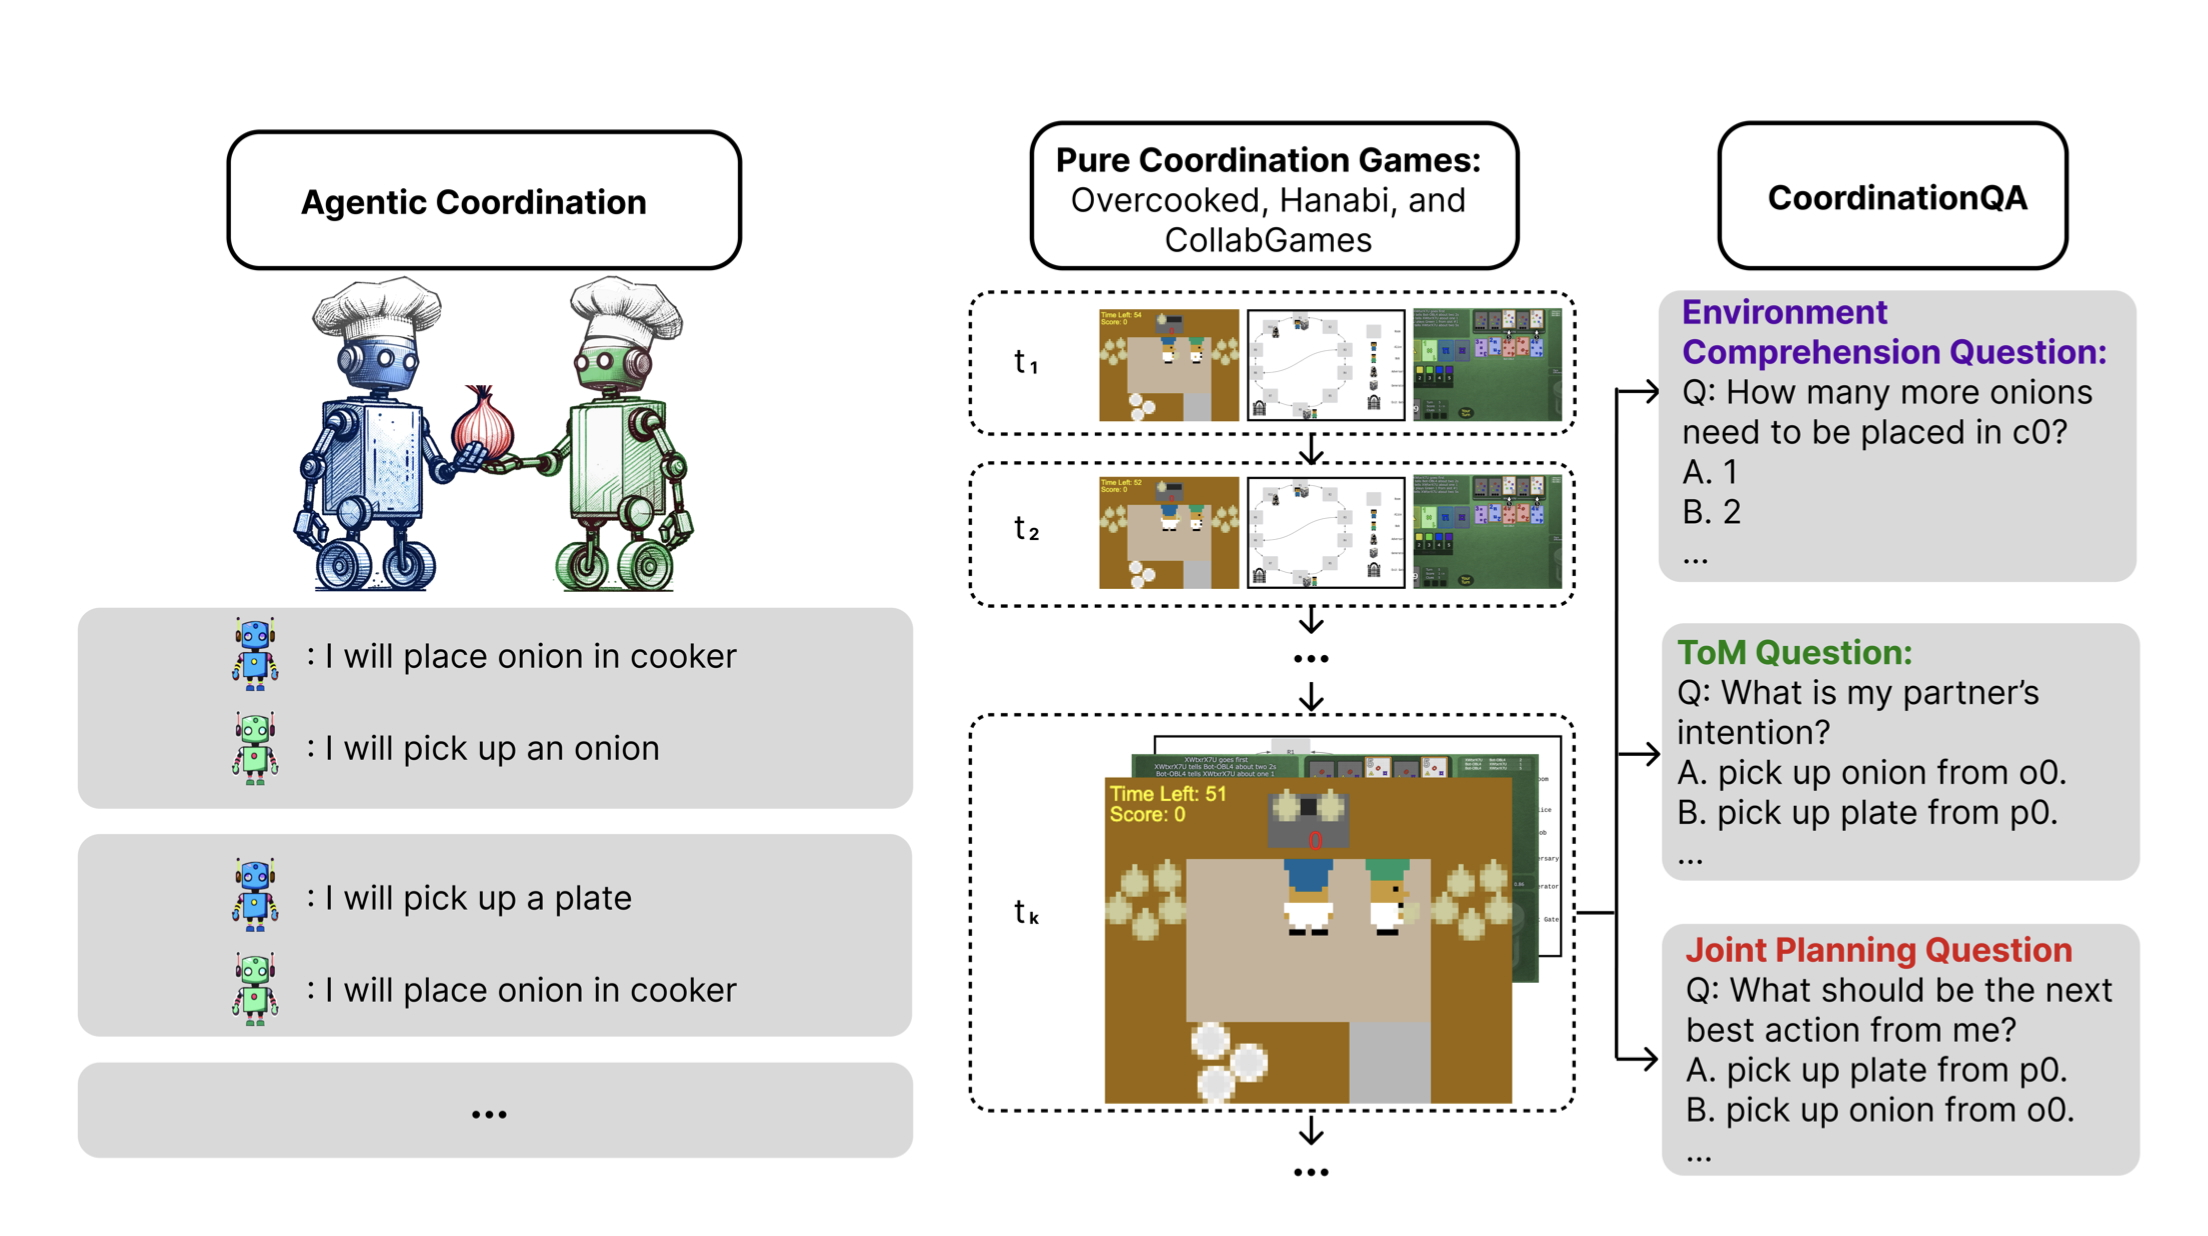
\includegraphics[width=14cm]{figures/llmcoordinationbank} 
    \caption{LLM 协调基准的图示 \citep{agashe2025llm}，它用两类度量来评估智能体式协调：在智能体必须合作以最大化收益的纯协调博弈中的行为（中），以及关于这些博弈的详细问题（右）}\label{fig:agashe}
  \end{center}
\end{figure}

纯合作博弈的关键特征是智能体必须彼此充分合作，没有任何竞争激励。相比之下，在囚徒困境（或 MAgIC 等基准中的混合动机博弈）这类竞争性设定中，智能体面临个体收益与集体收益之间的真实张力。在这类博弈中，当大语言模型未能合作时，原因并不清楚。该智能体可能是协调能力差，\textit{也可能}是在对个体收益作策略性推理。而在纯合作博弈中，任何时候都没有背叛的理由，因此任何合作失败都是协调能力的真正欠缺。

\subsection{单场景平台中的策略性交互}
基准是在许多小博弈上聚合。另一条互补的研究路线构建单一场景，深入考察智能体行为。

Alympics \citep{mao2023alympics} 提供了一个受控的游乐场，用于仿真由大语言模型驱动的智能体之间的策略性交互，以一个多轮水资源分配挑战为例——稀缺的生存资源必须随时间分配，见图~\ref{fig:water}。
\begin{figure}
  \begin{center}
    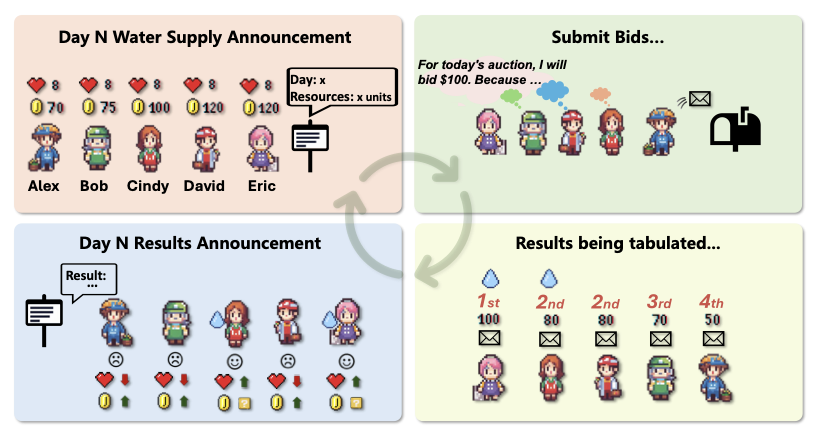
\includegraphics[width=13cm]{figures/water}
    \caption{Alympics 水资源分配
    挑战博弈 \citep{mao2023alympics}}\label{fig:water}
  \end{center}
\end{figure}

AucArena \citep{chen2023put} 仿真拍卖，横跨 LLaMa 2.13b、Mistral 7b、Mixtral 8x7b、Gemini 1.0 与 GPT 3.5/4.0，发现 GPT-4 等最强的大语言模型具备参与拍卖的技能，如预算管理与目标聚焦，不过即便对该模型而言表现也有波动，作者指出仍有相当大的改进空间。

\subsection{结论}
无论在基准还是单场景平台中，协调都一致地表现为大语言模型智能体的弱点。更强的大语言模型在 MAgIC 中理性与判断得分高，在 AucArena 中能合理管理预算，在环境驱动的合作中能追平训练过的强化学习智能体。然而，当成功需要推理搭档相信什么、意图什么时，除最强、脚手架最重的模型外，所有模型都失败了。

换言之，模型无法一致地把心理理论推理\emph{整合}进自身行为。在第~\ref{chap:behavior} 章中，这类失败被称为知行差距或字面—功能差距：GPT-4 在被提示预测巴赫或斯特拉文斯基中的交替模式时能准确回应，但对局时却无法付诸实施。不过，此处综述的多智能体研究让这一诊断变得更复杂。在 LLM 协调基准的提问部分中，关于联合规划的问题恰恰就是智能体在博弈每一步所面对的决策。而正是在这些问题上，模型表现最差（在心理理论问题上也好不了多少）。问答得分与跨博弈的智能体表现正相关。换言之，在这里「知」与「行」是一起动的：模型行动差的地方，当把行动问题直接摆到它面前时，它推理也差。因此对纯协调任务而言，缺陷在于采取搭档视角（心理理论）与联合规划本身，而不在于把推理转化为行动。

在另一个层面上，知行差距又出现了。在 Hanabi 中，GPT-4-turbo 只有在用显式的心理理论推理与自我验证步骤加脚手架时才能达到合理表现。没有这些，它在每一次 Hanabi 试验中都会犯致命错误。换言之，它最初行动错误，但在被提示检查推理与验证步骤时能识别并纠正这些错误。类似的性能提升也由 MAgIC 中的概率图建模、以及第~\ref{chap:behavior} 章讨论的策略行为研究中的社会思维链带来。{\em 大语言模型无法推理他人}与{\em 大语言模型不会自发部署这类推理}之间的界线显然很薄，而以结构化推理与验证步骤形式的智能体式嵌入，能把后者激发出来。

下一节考察对同一问题的另一种互补回应：与其升级智能体的推理，不如通过分配角色来构造交互本身。


\section{基于角色的任务求解与团队协作}\label{sec:roletask}
上一节中，智能体是对称的同侪，协调必须从它们自身的策略推理中涌现（成效有限）。本节讨论的研究中，协调是通过交互协议与分配具有不同目标的角色而\emph{设计在内}的。

就第~\ref{fivedimensions} 节定义的五个维度而言，这些研究改变\emph{策略}与\emph{结构}，同时保持总体交互类型为合作。我们从最简单走向最复杂的结构：互补配对、多方辩论、团队，以及压力下的社会角色扮演。

\subsection{互补配对}
大语言模型可以在被赋予互补角色的配对中执行任务，例如创建者—批评者或管理者—工作者。在这类成对设置中，每个大语言模型智能体被赋予一个不同的角色与目标，它们通过交流共同求解任务。

在 CAMEL 框架（用于「心智」探索的交流式智能体）\citep{li2023camel} 中，两个大语言模型各自扮演预定义角色，共同完成编程任务之类的目标（见图~\ref{fig:camel}）。通过合作，它们共同驱动一场对话，而无需人类持续显式提示。CAMEL 使用初始提示与角色描述，使智能体保持角色设定并朝向目标协作。智能体被提示通过对话把复杂问题拆解为可管理的步骤。在每个交互步骤中，大语言模型智能体实际上在生成自己的推理时训练数据，使认知过程对人类检视可见，同时增强自主任务表现。

\begin{figure}
  \begin{center}
    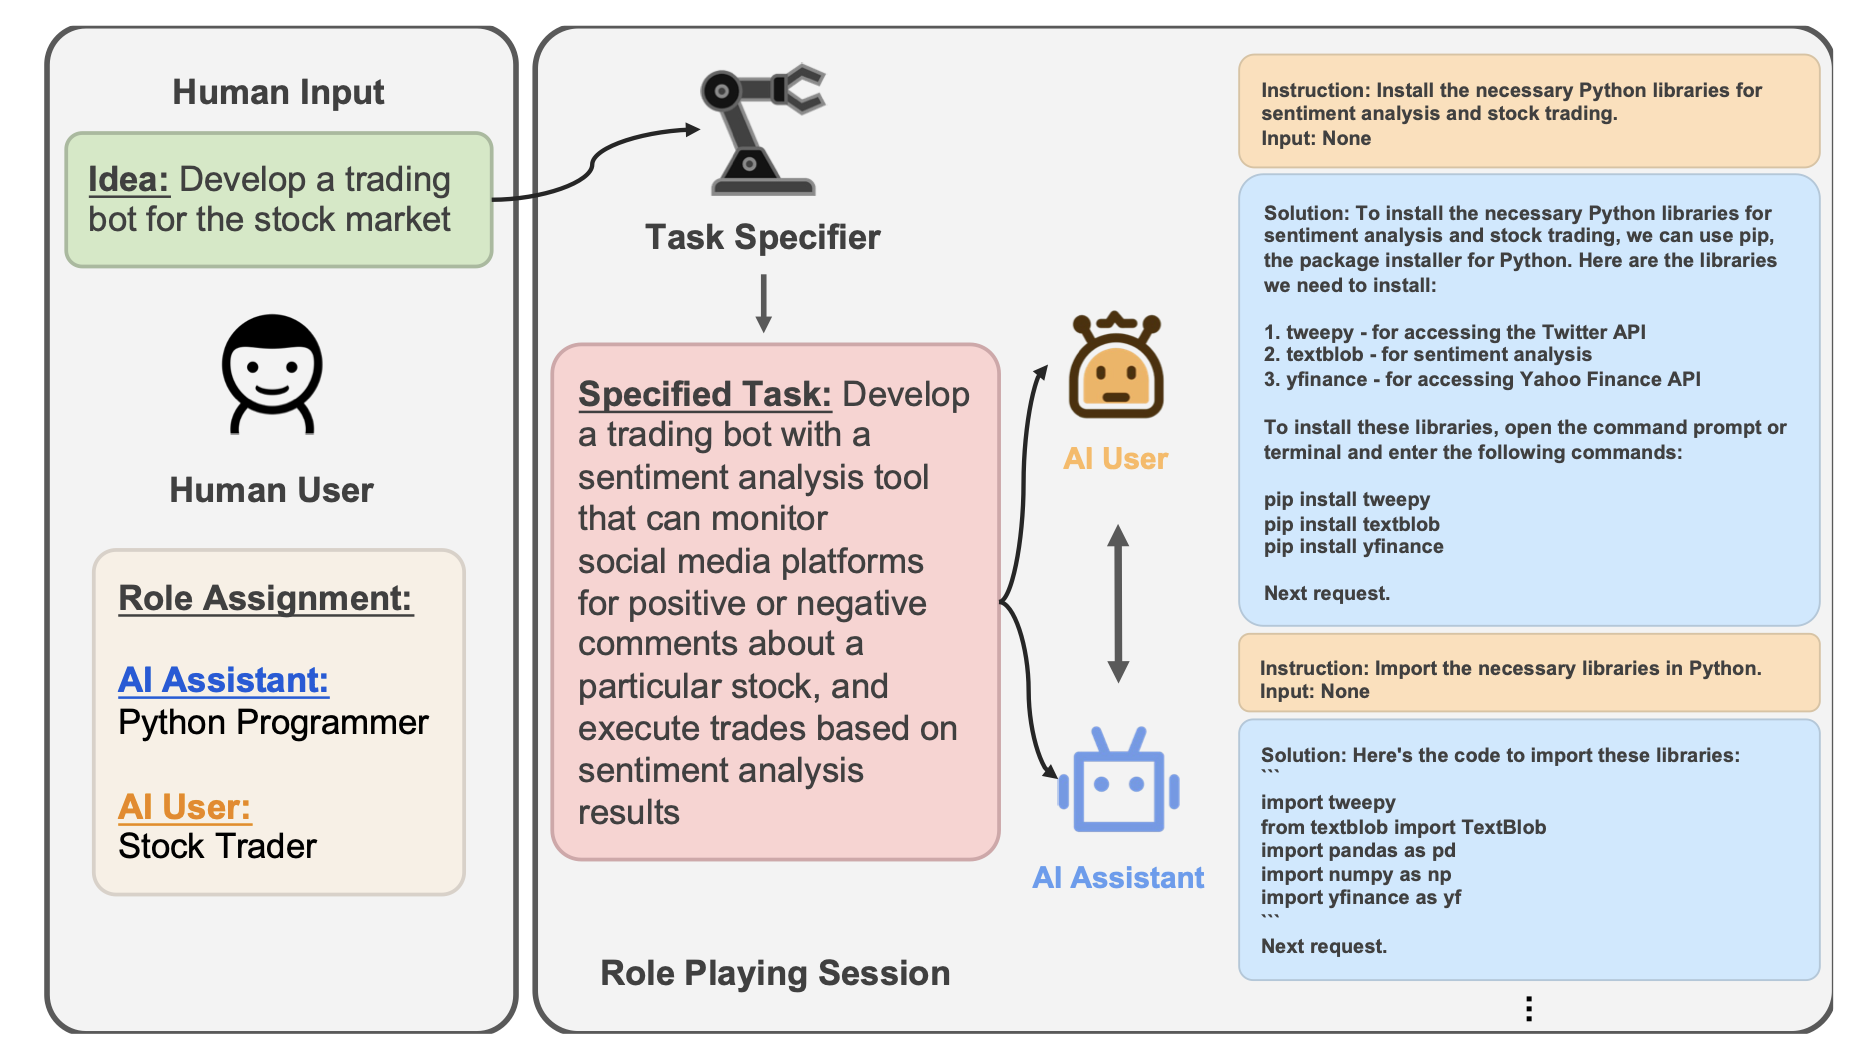
\includegraphics[width=\textwidth]{figures/CAMEL}
    \caption{CAMEL 中的角色扮演 \citep{li2023camel}}\label{fig:camel} 
  \end{center}
\end{figure}

其他研究把大语言模型创建者（或生成器）与一个大语言模型评判者（或批评者）配成一对，置于自反思设定中。这样，大语言模型的生成能力通过一个智能体发挥，而对规则或质量准则的遵守由另一个智能体强制。宪法式 AI \citep{bai2022constitutional} 用一个语言模型依据一套伦理或质量准则批评另一个语言模型的回应，并提出修改建议。作者表明，这类双智能体反馈能产出经过精炼、符合预期原则的最终输出。

第三种成对交互形式遵循人类辅导的动力学：教师—学习者或专家—新手。第~\ref{sec:distillation} 章在蒸馏语境中讨论了这一结构的各种例子。

三种配对都利用了同一想法：一个智能体的监督可以纠正另一个智能体的错误，从而带来比任一智能体单独所能达到的更稳健的联合表现。

\subsection{辩论与讨论}
在配对之外，基于角色交互的一个突出例子是用大语言模型之间的辩论与讨论来改善推理与任务表现。

\citet{du2024debate} 证明，当多个大语言模型实例提出答案并通过若干轮辩论相互批评彼此的推理时，它们能达成更准确、事实正确性更高的共识答案。这一方法被用明斯基的「心智社会」 \citep{minsky1988society} 来表述，在数学文字题与事实问答等任务中显著减少了推理错误与幻觉。

\citet{liang-etal-2024-encouraging} 提出多智能体辩论（MAD）设置：两个大语言模型智能体在诸如针锋相对的谈判中分居对立两方（见第~\ref{sec:strategic} 节），而第三个智能体充当评判者。评判者的作用是把讨论引向最终解法。这种结构化辩论鼓励发散思维，能推动一个经 MAD 增强的较弱模型（如 GPT-3.5）在某个高难度基准上超过未经 MAD 的更强模型（如 GPT-4）。作者讨论了他们的 MAD 设置如何克服自反思步骤加脚手架中的一个已知问题。自反思可能诱发所谓的\emph{思维退化}：一旦模型对某个解法方向产生信心，自反思会强化这种信心，即便该方向是错的。在 MAD 辩论设置中，另一个智能体可以把它推向不同方向，以避免思维退化。

ChatEval 把这一辩论模式应用于文本评测 \citep{chan2023chateval}。作者注意到当多个标注者协作时人类文本评估的质量会提升，于是构建了一个多智能体评审团，包含辩手智能体、多样化的角色设定与不同的交流策略（见图~\ref{fig:chateval}），超越了单智能体提示策略。

\begin{figure}
  \begin{center}
    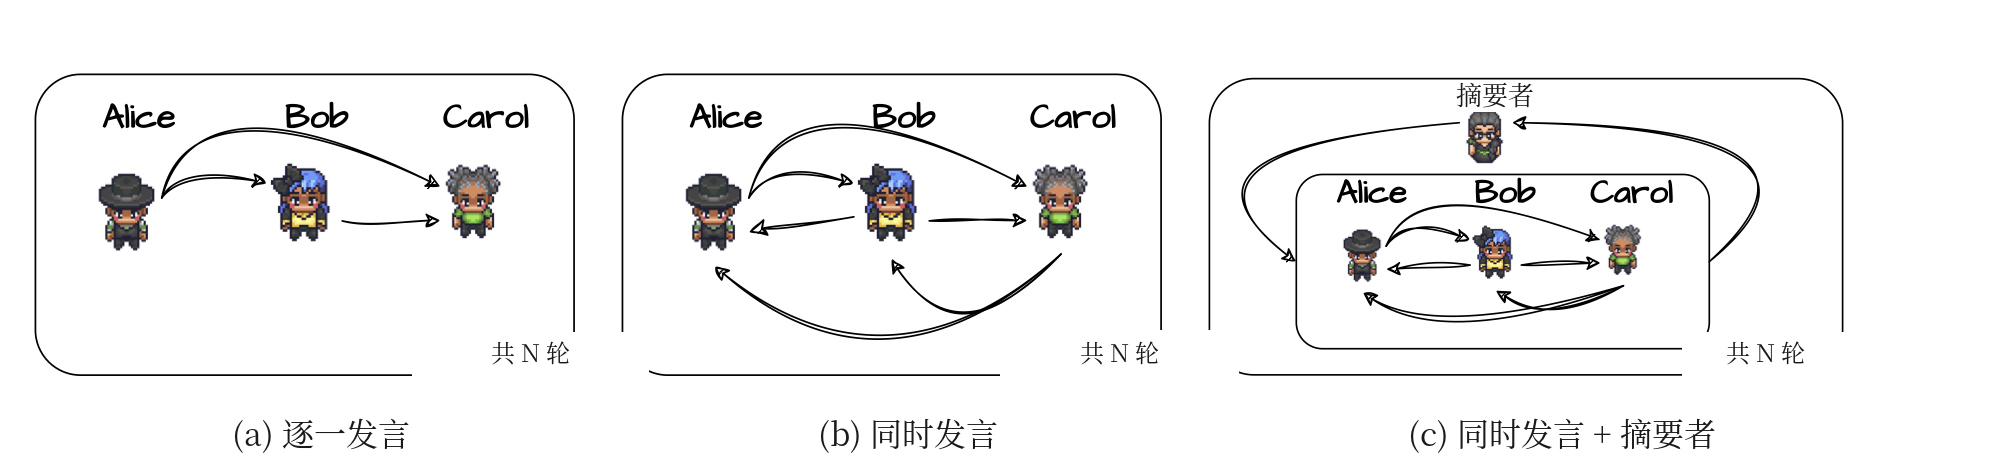
\includegraphics[width=14cm]{figures/chateval}
    \caption{ChatEval 中的三种不同交流策略 \citep{chan2023chateval}}\label{fig:chateval} 
  \end{center}
\end{figure}

另一种同样受明斯基「心智社会」启发的做法是 ReConcile，这是一个被设计为多样大语言模型智能体之间圆桌会议的多智能体框架 \citep{chen2023reconcile}。该框架通过多轮讨论增强大语言模型智能体之间的协作推理。智能体必须试图说服彼此以改进答案。在七个基准上的实验表明，置信度加权投票机制显著改善了大语言模型的推理。此外，作者发现多样性（使用不同的底层模型）对表现至关重要。

MindStorms 引入了基于大语言模型的实现 \citep{zhuge2023mindstorms}，建立在 CAMEL 框架 \citep{li2023camel} 之上。报告了大量实验，最多用到 129 个智能体来求解常见人工智能问题：视觉问答、图像描述、文本到图像合成、3D 生成、自我中心检索、具身人工智能，以及一般性的基于语言的任务求解。作者发现，在特定应用中，成员更多的头脑风暴优于成员更少的，更长的头脑风暴优于更短的。

\subsection{基于角色的软件团队}
基于角色协作的一个有趣应用是软件开发——由大语言模型智能体完全充任的仿真团队来开发软件。

大语言模型的自动化编程一直受困于逻辑不一致、以及在整个开发流水线中级联的幻觉等问题。MetaGPT \citep{hong2024metagpt} 建立在已被证明在人类软件团队中有效的工作流之上。该框架把标准作业流程（SOP）转换成提示词序列，并把智能体分配为一家软件公司的角色：产品经理、架构师、工程师、QA 测试员。这样，智能体沿流水线向下传递结构化的中间产物。产品经理写出需求文档，架构师把它转成设计，工程师写代码。如此，复杂任务被划分为可管理的子任务，智能体可以逐步验证过程，显著减少错误。

类似地，\citet{qian-etal-2024-chatdev} 提出了 ChatDev，一家虚拟软件公司，智能体在开发过程的各个阶段（设计、编码、测试）协作。协作被组织为一条\emph{对话链}：每个阶段被分解为指导者与助手智能体之间的简短对话（见图~\ref{fig:chatdev2}）。使用一种让智能体在回应前先索要更多细节的通信协议，带来了作者所称的\emph{去幻觉}，提高了每一步的可靠性。该框架展示了自然语言中的结构化通信如何促进多智能体协作。

\begin{figure}
  \begin{center}
    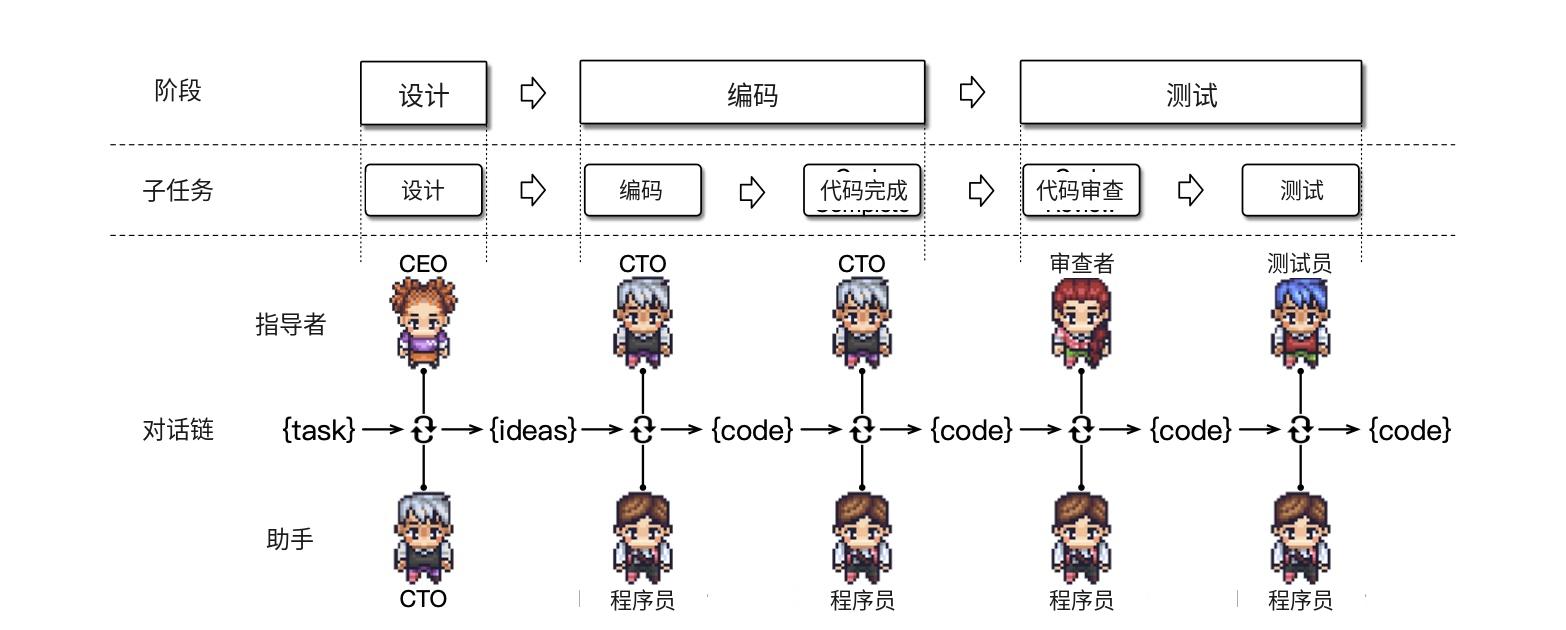
\includegraphics[width=14cm]{figures/chatdev2.jpg}
    \caption{ChatDev 中基于 ChatGPT-3.5 驱动的智能体之间多轮二元通信的链式结构工作流 \citep{qian-etal-2024-chatdev}}\label{fig:chatdev2} 
  \end{center}
\end{figure}

MetaGPT 与 ChatDev 把特定组织结构硬编码，而 AutoGen \citep{wu2024autogen} 提供了一个灵活的编程框架，基于可定制智能体之间的对话，这些智能体可以组合大语言模型、工具与人类输入。它被设计为一个开源平台，让开发者依据应用来定义智能体与交互结构。实验证明了它在数学、编程、问答、娱乐等领域任务上的有效性。


\subsection{社会角色扮演}
上面讨论的系统分配角色是为了求解任务。最后一条研究路线分配角色是为了研究社会行为本身：当大语言模型智能体被置于社会要求高或存在冲突的情境中时，它们会做什么？

\begin{figure}
  \begin{center}
    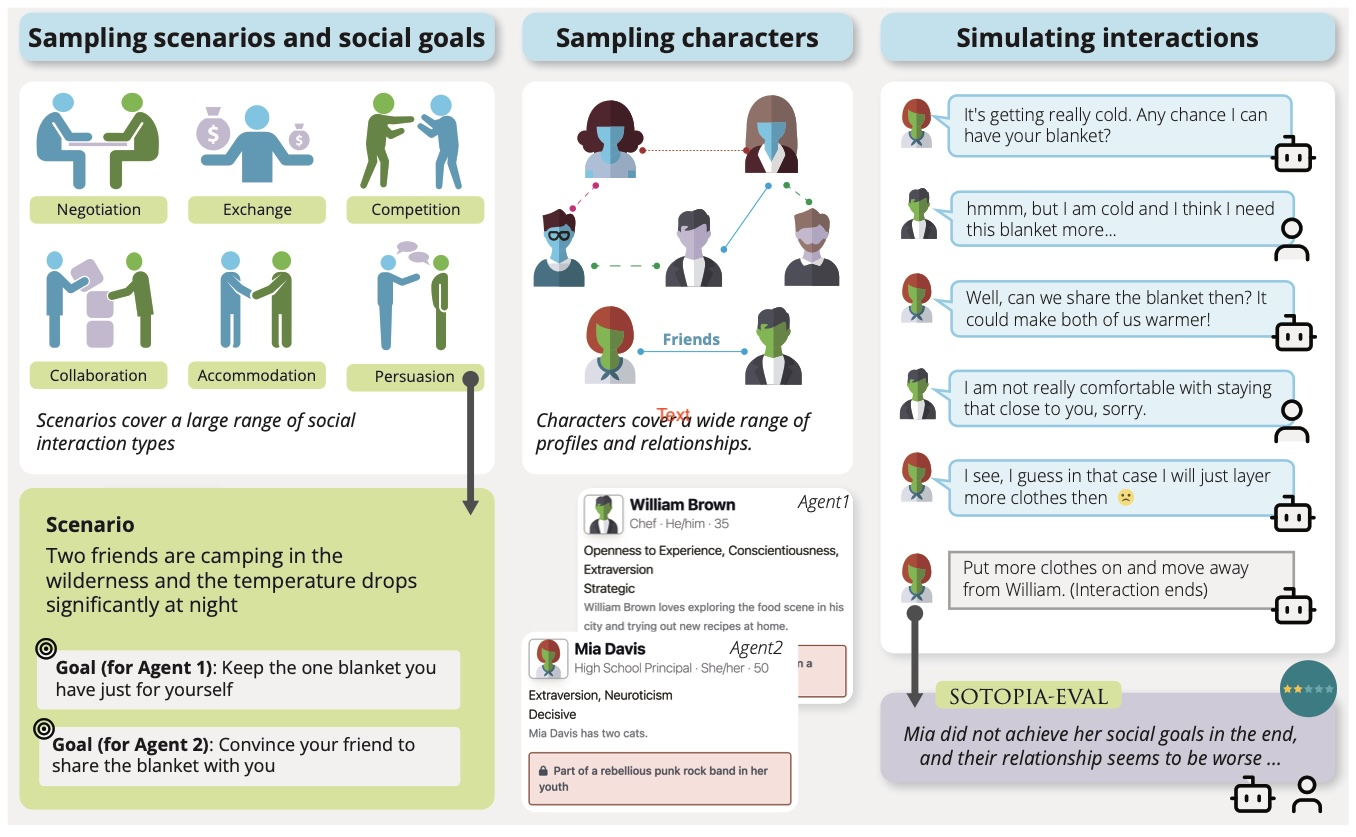
\includegraphics[width=14cm]{figures/sotopia.jpg}
    \caption{SOTOPIA 中一个具有冲突性社会目标的场景图示 \citep{zhou2023sotopia}}\label{fig:sotopia} 
  \end{center}
\end{figure}

在 SOTOPIA \citep{zhou2023sotopia} 中，智能体协调、协作与竞争以实现复杂的社会目标。SOTOPIA 环境从 90 个（自动生成的）社会场景中采样\emph{交互片段}，涵盖 40 个具有各自人格、职业、秘密、背景故事及彼此关系的角色，从而形成一个大而多样的任务空间（图~\ref{fig:sotopia}）。作者基于不同大语言模型评估智能体的社会智力，并与人类参与者相比，观察到若干趋势：
\begin{itemize}
    \item 在涉及社会推理的静态基准（如 ToMBench，见第~\ref{sec:theoryofmind} 节）上表现良好的模型，未必能在交互式场景中成功，这再次体现了知行差距（第~\ref{sec:strategic} 节）。
    \item 较弱的智能体会削弱其对话伙伴，这与上面讨论的会话优势恰好相反——在那里，智能体阻止了彼此产生思维退化等错误。
    \item 泄露秘密与违反社会规范在所有模型中都被观察到，与道德行为语境中讨论的观察一致（第~\ref{sec:moral} 节）。\
    \item 在最困难的 SOTOPIA 任务上，人类的表现显著优于即便是表现最好的模型（GPT-4）。
\end{itemize}
作者主张，SOTOPIA 的动态与交互特性给大语言模型智能体带来了静态基准系统性地无法揭示的独特挑战。

极端设定下的社会交互在 \citep{campedelli2024want} 中得到研究。受臭名昭著的斯坦福监狱实验 \citep{zimbardo1972stanford} 启发，作者考察在囚犯与狱警的设定中说服性与虐待性行为的涌现。研究发现，被赋予的囚犯与狱警人格既影响说服力，也影响反社会行为的涌现。关键在于，这表明反社会行为可以通过角色分配与特定交互环境在大语言模型智能体中涌现。这与原始的人类参与者实验形成了惊人的平行，并再次提醒我们注意模型如何判断情境（通常反映人口平均的道德规范）与智能体一旦被投入特定行动语境后如何行为之间的差距（另见第~\ref{sec:moral} 节）。该研究还发现，角色分配并非中立的工程工具：它可以以不良方式塑造行为。

为仿真合作设定中的策略性决策，研究者提出了 GovSim \citep{piatti2024cooperate}。他们研究伦理考量、战略规划与谈判技能如何影响合作结果。多数大语言模型无法达成均衡，因为它们未能理解自身行动对群体的长期影响。有趣的是，引入一种特殊的\emph{普遍化}推理语言 \citep{levine2020logic}（提示模型提出康德式问题：\emph{如果每个人都这样做呢？}）让更多模型达成了可持续的结果。\citet{bianchi2024well} 提出的 NegotiationArena 中展示了相关结果。他们表明大语言模型智能体能在谈判场景中通过灵活对话进行复杂谈判。灵活对话通过采用不同行为策略显著改善了谈判结果。

\subsection{结论}
本节的研究回应第~\ref{sec:strategic} 节所识别的协调弱点的方式，不是让单个智能体成为更好的推理者（如第~\ref{sec:enhancement} 节），而是构造它们周围的交互。互补角色告诉每个智能体它应有何贡献，而交互协议与 SOP 规范智能体何时、以何种形式通信。在某些设置中，评判者或投票机制有助于把分歧引向有成效的解决。

当内部协调本会不足时，角色与交互协议提供了关键的脚手架。这可以看作第~\ref{chap:behavior} 章讨论的结构化推理方案（如社会思维链、概率图，或围绕道德规则的审议）在多智能体中的对应物。这些方案在不受约束的推理无法奏效时提升了表现。无论在单智能体还是多智能体情形中，模型的潜在（社会、道德等）知识与行为都是真实存在的，但需要通过显式结构来激活。

% Related to debate and discussion setups, researchers have explored teacher-learner dynamics with LLMs, where an expert LLM provides hints or feedback to a less capable LLM, mirroring human tutoring \citep{zhou2023sotopia}. These role-alignments leverage the same idea as the MAD setup: one agent’s oversight can correct the other’s mistakes, leading to more robust performance and a lower chance of falling into thought-degeneration loop holes. 
%AutoGen \citep{wu2023autogen} is designed to facilitate the development of multi agent LLM applications that span a broad spectrum of domains and complexities. The programming paradigm is centered around agent-agent conversations. Experiments demonstrate the effectiveness of the framework in  example applications ranging from mathematics, coding, question answering, operations research, online decision-making, to entertainment.

% Sotopia is another role-playing environment for multi-agent interaction \citep{zhou2023sotopia}. In Sotopia, agents coordinate, collaborate, exchange, and compete with each other to achieve complex social goals. In experiments with LLM-agents and humans,  GPT-4 achieves a significantly lower goal completion rate than humans and struggles to exhibit social commonsense reasoning and strategic communication skills. The contrast between GPT-4's lower performance in Sotopia and good performance on other metrics of social reasoning (see Section \ref{sec:tom}) is most likely explained by Sotopia's focus on strategizing and goal-directedness, aspects on which GPT-4 has been reported to score lower \citep{hou2024entering}.

\section{结语}
本章从大语言模型智能体在策略博弈中彼此对阵，经由基于角色的协作模式与实践中协调它们的多种设置，直到对多智能体系统何时奏效、何时失败的批判性评估。

在第~\ref{chap:behavior} 章中，我们发现单个模型协调能力差，并且能在形式上预测搭档会做什么，却在智能体式实现中不依据该预测行动。这两种模式都迁移到了多智能体设定。跨基准与平台（如 \citep{xu2024magic, agashe2025llm}），交互中的大语言模型智能体能就自利进行推理，却无法协调自身行为，从而把这种推理转化为策略优势。一个主要问题是它们能否依据搭档的视角来调整行为，这一问题在第~\ref{sec:theoryofmind} 节讨论的心理理论的知行或字面—功能能力差距中已有预兆。这与系统性地把智能体间错位识别为多智能体系统主要失效类别的工作相呼应 \citep{cemri2025masfail}。

这个字面—功能问题再次与构念效度相关：正如通过一项心理理论测试并不能确立人类级别的社会推理能力，一个多智能体设置在单次大语言模型查询上取得更优表现，也不能确立集体智能。强基线、匹配的推理预算，以及对协作结构与交互协议的消融实验，将是第~\ref{sec:theoryofmind} 节讨论的扰动式心理理论测试在多智能体中的对应物。多智能体领域需要更多研究，才能就智能体式大语言模型交互的现状建立扎实的实证图景。

最后，多智能体设定带来了新的风险类别。角色分配被证明能够在一个受斯坦福监狱实验启发的设定中激活反社会乃至虐待性行为 \citep{campedelli2024want}。在其他研究中，协调失当、级联幻觉与弱点的相互强化，触发了规范违反、秘密泄露与任务表现下降。在有些情况下，指定角色与交互协议为行为加了脚手架并提升了表现；在另一些情况下，它们却成了障碍或风险来源。

下一章我们讨论那些不分配角色与协议、而让它们从交互本身中涌现的研究。


\bibliographystyle{plainnat}
\bibliography{agenticbook,refs,case,synthetic}
